\documentclass{article}
\usepackage[margin=3.5cm]{geometry}   
\usepackage{tikz,amsmath}
\usepackage{pgfgantt}
\usepackage{lscape}
\usepackage{rotating}
\usetikzlibrary{arrows,shapes,positioning,shadows,trees}
\usepackage[
  colorlinks=true,
  urlcolor=cyan!70!black
  ]{hyperref}
	
\title{Homework II}
\author{Gregory Williams\\GW4975\\EE 382C Program Management}
\date{10/09/2015}

\begin{document}
	\maketitle
	\section*{Problem 9.14}
	
	\begin{center}
	\makebox[\textwidth]{
		
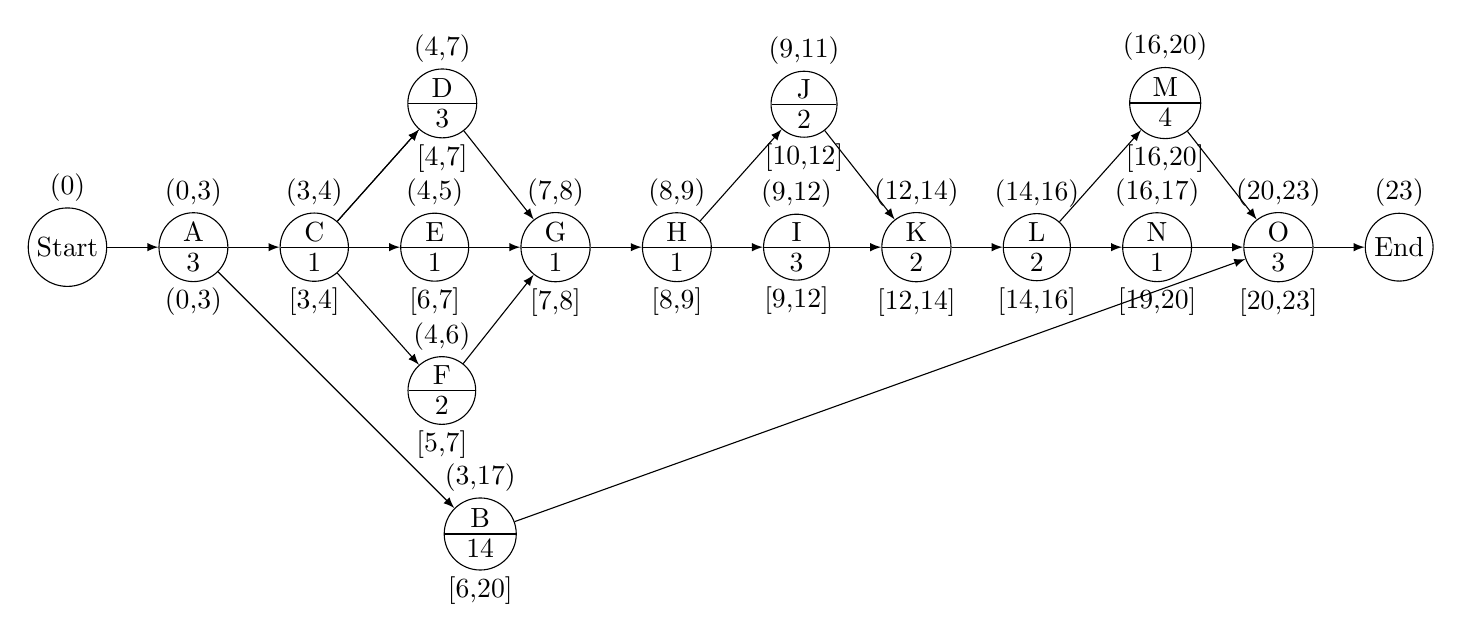
\begin{tikzpicture}[
  >=latex,
  every node/.style={draw,inner sep=2pt,minimum size=1pt},
  scale=0.5,
  node distance=.65cm,
  ]
  \node[circle, label=90:(0),] (S){Start};
  \node[circle split, right = of S, label=90:{(0,3)}, label=270:{(0,3)}] (A) {A \nodepart{lower} 3};
  \node[circle split, below right = 3 and 3 of A, label=90:{(3,17)}, label=270:{[6,20]}] (B) {B \nodepart{lower} 14};
  \node[circle split, right = of A, label=90:{(3,4)}, label=270:{[3,4]}] (C) {C \nodepart{lower} 1};
  \node[circle split, above right = 1.2 and 1 of C, label=90:{(4,7)}, label=270:{[4,7]}] (D) {D \nodepart{lower} 3};
  \node[circle split, right = of C, label=90:{(4,5)}, label=270:{[6,7]}] (E) {E \nodepart{lower} 1};
  \node[circle split, below right = 1.2 and 1 of C, label=90:{(4,6)}, label=270:{[5,7]}] (F) {F \nodepart{lower} 2};
  \node[circle split, right = of E, label=90:{(7,8)}, label=270:{[7,8]}] (G) {G \nodepart{lower} 1};
  \node[circle split, right = of G, label=90:{(8,9)}, label=270:{[8,9]}] (H) {H \nodepart{lower} 1};
  \node[circle split, right = of H, label=90:{(9,12)}, label=270:{[9,12]}] (I) {I \nodepart{lower} 3};
  \node[circle split, above right = 1.2 and 1 of H, label=90:{(9,11)}, label=270:{[10,12]}] (J) {J \nodepart{lower} 2};
  \node[circle split, right = of I, label=90:{(12,14)}, label=270:{[12,14]}] (K) {K \nodepart{lower} 2};
  \node[circle split, right = of K, label=90:{(14,16)}, label=270:{[14,16]}] (L) {L \nodepart{lower} 2};
  \node[circle split, above right = 1.2 and 1 of L, label=90:{(16,20)}, label=270:{[16,20]}] (M) {M \nodepart{lower} 4};
  \node[circle split, right = of L, label=90:{(16,17)}, label=270:{[19,20]}] (N) {N \nodepart{lower} 1};
  \node[circle split, right = of N, label=90:{(20,23)}, label=270:{[20,23]}] (O) {O \nodepart{lower} 3};
  \node[circle, right = of O, label=90:{(23)}] (End) {End};
  
  
  \draw [->] (S) -- (A);
  \draw [->] (A) -- (B);
  \draw [->] (A) -- (C);
  \draw [->] (C) -- (D);
  \draw [->] (C) -- (E);
  \draw [->] (C) -- (F);
  \draw [->] (D) -- (G);
  \draw [->] (E) -- (G);
  \draw [->] (F) -- (G);
  \draw [->] (G) -- (H);
  \draw [->] (H) -- (I);
  \draw [->] (H) -- (J);
  \draw [->] (C) -- (D);
  \draw [->] (I) -- (K);
  \draw [->] (J) -- (K);
  \draw [->] (K) -- (L);
  \draw [->] (L) -- (M);
  \draw [->] (L) -- (N);
  \draw [->] (B) -- (O);
  \draw [->] (M) -- (O);
  \draw [->] (N) -- (O);
  \draw [->] (O) -- (End);
  
\end{tikzpicture}

}
	\end{center}
	Critical path: A-C-D-G-H-I-K-L-M-O \\
	Duration: 23 days
	\pagebreak
	\section*{Problem 9.15}
	
	{\renewcommand{\arraystretch}{1.2} 
	\begin{table}[h!tbp]
  		\begin{center}
    		\caption{Slacks for Buying Tom Cruise a Boat}
    		\label{tab:table1}
			
    		\begin{tabular}{lcccccc}
				 & Total Slack Eq &  &  & Free Slack Eq & &\\
				Activity & LS - ES & = & Total Slack & Min\{ES$_{\text{Suc}}$\} - EF &= & Free Slack \\
				\hline
      			A* & & &0 & & &0\\
      			B & 20-17&= & 3 & 20-17&= & 3\\
				C* &&& 0 &&& 0\\
				D* &&& 0 &&& 0\\
				E & 6-4&= & 2 & 7-5&= & 2\\
				F & 5-4&= & 1 & 7-6&= & 1\\
				G* &&& 0 &&& 0\\
				H* &&& 0 &&& 0\\
				I* &&& 0 &&& 0\\
				J & 10-9&= & 1 & 12-11&= & 1\\
				K* &&& 0 &&& 0\\
				L* &&& 0 &&& 0\\
				M* &&& 0 &&& 0\\
				N & 19-26&= & 3 & 20-17&= & 3\\
				O* &&& 0 &&& 0\\
				\hline
				\multicolumn{3}{c}{* = On the Critical Path}\\
    		\end{tabular}
  		\end{center}
	\end{table}
	}
	
	\section*{Problem 9.19}
	\subsection*{(a)}
	\begin{center}
	\makebox[\textwidth]{
		
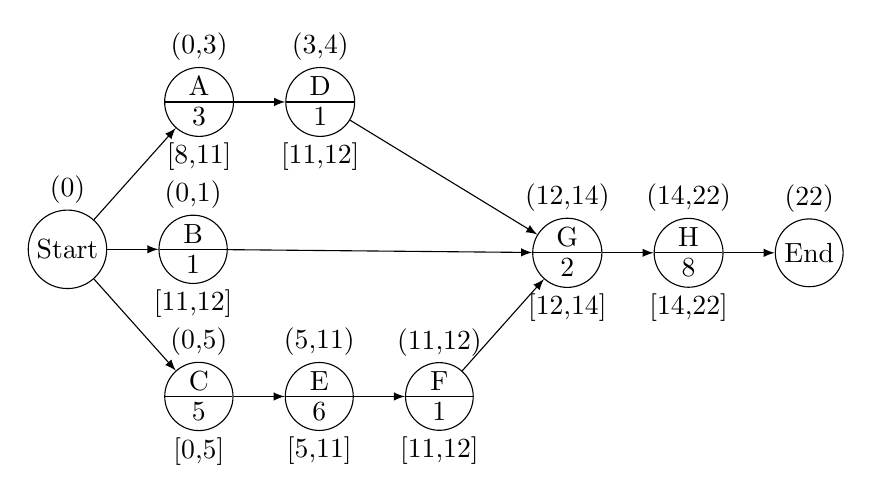
\begin{tikzpicture}[
  >=latex,
  every node/.style={draw,inner sep=2pt,minimum size=1pt},
  node distance=.65cm,
  ]
  \node[circle, label=90:(0),] (S){Start};
  \node[circle split, above right = 1.2 and 1 of S, label=90:{(0,3)}, label=270:{[8,11]}] (A) {A \nodepart{lower} 3};
  \node[circle split, right = of S, label=90:{(0,1)}, label=270:{[11,12]}] (B) {B \nodepart{lower} 1};
  \node[circle split, below right = 1.2 and 1of S, label=90:{(0,5)}, label=270:{[0,5]}] (C) {C \nodepart{lower} 5};
  \node[circle split, right = of A, label=90:{(3,4)}, label=270:{[11,12]}] (D) {D \nodepart{lower} 1};
  \node[circle split, right = of C, label=90:{(5,11)}, label=270:{[5,11]}] (E) {E \nodepart{lower} 6};
  \node[circle split, right = of E, label=90:{(11,12)}, label=270:{[11,12]}] (F) {F \nodepart{lower} 1};
  \node[circle split, above right = 1.2 and 1of F, label=90:{(12,14)}, label=270:{[12,14]}] (G) {G \nodepart{lower} 2};
  \node[circle split, right = of G, label=90:{(14,22)}, label=270:{[14,22]}] (H) {H \nodepart{lower} 8};
  \node[circle, right = of H, label=90:{(22)}] (End) {End};
  
  
  \draw [->] (S) -- (A);
  \draw [->] (S) -- (B);
  \draw [->] (S) -- (C);
  \draw [->] (A) -- (D);
  \draw [->] (C) -- (E);
  \draw [->] (E) -- (F);
  \draw [->] (B) -- (G);
  \draw [->] (D) -- (G);
  \draw [->] (F) -- (G);
  \draw [->] (G) -- (H);
  \draw [->] (H) -- (End);
  
\end{tikzpicture}

}
	\end{center}
	\pagebreak
	\subsection*{(b)}
	{\renewcommand{\arraystretch}{1.2} 
	\begin{table}[h!tbp]
  		\begin{center}
    		\caption{Slacks for Buying Tom Cruise a Boat}
    		\label{tab:table2}
			
    		\begin{tabular}{lcccccc}
				 & Total Slack Eq &  &  & Free Slack Eq & &\\
				Activity & LS - ES & = & Total Slack & Min\{ES$_{\text{Suc}}$\} - EF &= & Free Slack \\
				\hline
      			A & 8-0&= & 8 & 3-3&=& 0\\
      			B & 11-0&= & 11 & 12-1&= & 11\\
				C* && &0 &&& 0\\
				D & 11-3&= & 8 & 12-4&= & 8\\
				E* &&& 0 &&& 0\\
				F* &&& 0 &&& 0\\
				G* &&& 0 &&& 0\\
				H* &&& 0 &&& 0\\
				\hline
				\multicolumn{3}{c}{* = On the Critical Path}\\
    		\end{tabular}
  		\end{center}
	\end{table}
	}
	
	\noindent The total slack means that the activity may be delayed from the early start by that amount of time without affecting the total project duration; the free slack is the amount of time the activity may be delayed without delaying any other activity in the project.\\
	For this project, investigating the demand can be delayed for 8 weeks without affecting the overall project, but if it is delayed at all it will delay the conducting of the promotional cost analysis activity.\\
	The pricing strategy and the the conducting of the promotional cost analysis activities can be delayed for their total slack times without delaying any other activities, as their total slacks and free slacks are equal.
	
	\subsection*{(c)}
	Critical Path: C-E-F-G-H\\
	For this project, the design of the product must be completed before the manufacture of the prototype models. In turn, those models must be completed before the product cost analysis, final pricing analysis, and market test activities can be completed.\\
	This project appears to be dominated by the design, manufacture, and test of the product, which makes sense. Strategies and market analyses are useful, but ultimately worthless without a product to sell.
	\subsection*{(d)}
	\begin{center}
	\makebox[\textwidth]{
		
\begin{ganttchart}[vgrid,hgrid,
	bar/.append style={fill=blue!50},
	bar incomplete/.append style={fill=Maroon},
	]{1}{22}
  \gantttitle{Gantt Chart for 9.19}{22} \\
  \gantttitlelist{1,...,22}{1} \\
	\ganttbar{A}{1}{3}\\%\ganttbar{}{5}{6} \\ %LOL, just add another bar!
	\ganttbar{B}{1}{1} \\%\ganttbar[bar/.append style={fill=gray!30}]{}{4}{4} \\
	\ganttbar{C}{1}{5} \\%\ganttbar[bar/.append style={fill=gray!30}]{}{7}{7} \\
	\ganttbar{D}{4}{4} \\
	\ganttbar{E}{6}{11} \\%\ganttbar[bar/.append style={fill=white}]{}{9}{9} \\
	\ganttbar{F}{12}{12} \\
	\ganttbar{G}{13}{14} \\%\ganttbar[bar/.append style={fill=gray!30}]{}{11}{11}\\
	\ganttbar{H}{15}{22} 
\end{ganttchart}
}
	\end{center}
	
	\section*{Problem 9.20}
	\subsection*{(a)}
	
	{\renewcommand{\arraystretch}{1.2} 
	\begin{table}[h!tbp]
  		\begin{center}
    		\caption{Calculated Mean and Standard Deviation}
    		\label{tab:table3}
			
    		\begin{tabular}{lccccc}
				\hline
				&\multicolumn{3}{c}{Time estimate (weeks)} &&\\\cline{2-4}
				Activity & Optimistic & Most likely & Pessimistic & Mean & Std. Dev.\\
				\hline
				A & 1 & 3 & 4  & 2.83 & 0.5\\
				B & 1 & 1 & 2  & 1.17 & 0.17\\
				C & 4 & 5 & 9  & 5.50 & 0.83\\
				D & 1 & 1 & 1  & 1    & 0\\
				E & 4 & 6 & 12 & 6.67 & 1.33\\
				F & 1 & 1 & 2  & 1.17 & 0.17\\
				G & 1 & 2 & 3  & 2.0  & 0.33\\
				H & 6 & 8 & 10 & 8.0  & 0.67\\
				\hline
    		\end{tabular}
  		\end{center}
	\end{table}
	}
	
	\begin{center}
	\makebox[\textwidth]{
		
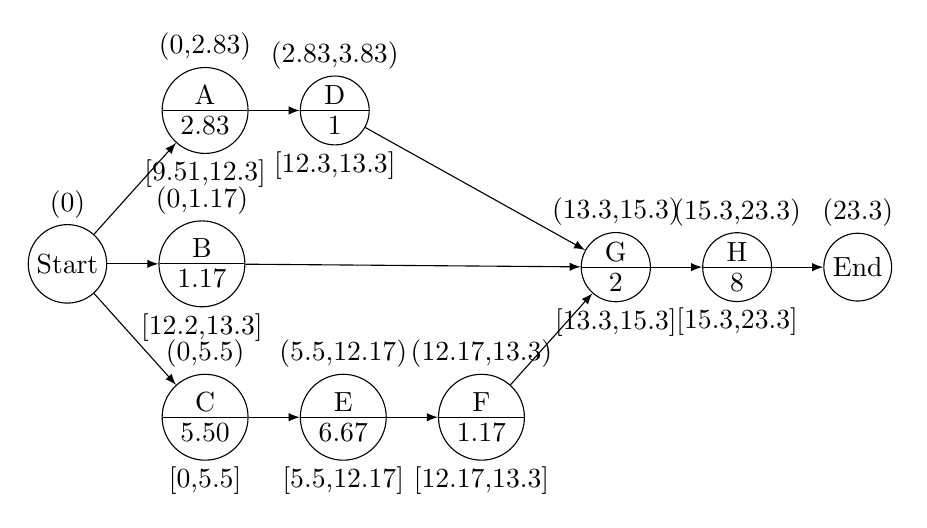
\begin{tikzpicture}[
  >=latex,
  every node/.style={draw,inner sep=2pt,minimum size=1pt},
  node distance=.65cm,
  ]
  \node[circle, label=90:(0),] (S){Start};
  \node[circle split, above right = 1.2 and 1 of S, label=90:{(0,2.83)}, label=270:{[9.51,12.3]}] (A) {A \nodepart{lower} 2.83};
  \node[circle split, right = of S, label=90:{(0,1.17)}, label=270:{[12.2,13.3]}] (B) {B \nodepart{lower} 1.17};
  \node[circle split, below right = 1.2 and 1of S, label=90:{(0,5.5)}, label=270:{[0,5.5]}] (C) {C \nodepart{lower} 5.50};
  \node[circle split, right = of A, label=90:{(2.83,3.83)}, label=270:{[12.3,13.3]}] (D) {D \nodepart{lower} 1};
  \node[circle split, right = of C, label=90:{(5.5,12.17)}, label=270:{[5.5,12.17]}] (E) {E \nodepart{lower} 6.67};
  \node[circle split, right = of E, label=90:{(12.17,13.3)}, label=270:{[12.17,13.3]}] (F) {F \nodepart{lower} 1.17};
  \node[circle split, above right = 1.2 and 1of F, label=90:{(13.3,15.3)}, label=270:{[13.3,15.3]}] (G) {G \nodepart{lower} 2};
  \node[circle split, right = of G, label=90:{(15.3,23.3)}, label=270:{[15.3,23.3]}] (H) {H \nodepart{lower} 8};
  \node[circle, right = of H, label=90:{(23.3)}] (End) {End};
  
  
  \draw [->] (S) -- (A);
  \draw [->] (S) -- (B);
  \draw [->] (S) -- (C);
  \draw [->] (A) -- (D);
  \draw [->] (C) -- (E);
  \draw [->] (E) -- (F);
  \draw [->] (B) -- (G);
  \draw [->] (D) -- (G);
  \draw [->] (F) -- (G);
  \draw [->] (G) -- (H);
  \draw [->] (H) -- (End);
  
\end{tikzpicture}

}
	\end{center}
	\subsection*{(b)}
	{\renewcommand{\arraystretch}{1.2} 
	\begin{table}[h!tbp]
  		\begin{center}
    		\caption{Slacks for Buying Tom Cruise a Boat}
    		\label{tab:table2}
			
    		\begin{tabular}{lcccccc}
				 & Total Slack Eq &  &  & Free Slack Eq & &\\
				Activity & LS - ES & = & Total Slack & Min\{ES$_{\text{Suc}}$\} - EF &= & Free Slack \\
				\hline
				\hline
      			A  & 9.51-0&= & 9.51 & 2.83-2.83&=& 0\\
      			B  & 12.2-0&= & 12.2 & 13.3-1.1&= & 12.2\\
				C* &       & &0 && 0\\
				D  & 12.3-2.83&= & 9.51 & 13.3-3.83&= & 9.51\\
				E* && &0 && 0\\
				F* && &0 && 0\\
				G* && &0 && 0\\
				H* && &0 && 0\\
				\hline
				\multicolumn{3}{c}{* = On the Critical Path}\\
    		\end{tabular}
  		\end{center}
	\end{table}
	}
	\subsection*{(c)}
	\noindent Critical Path: C-E-F-G-H\\
	Critical Path Mean Duration: 23.3 weeks\\
	Critical Path Standard Deviation: $[0.83^2 + 1.33^2 + 0.17^2 + 0.33^2 + 0.67^2]^{1/2} = 1.75$
	\\
	
	\noindent The critical path activities have not changed, but the expected total duration has increased to 23.3 weeks from 22 weeks. 
	\subsection*{(d)}
	
	\subsubsection*{(1)}
	\begin{equation*}
		P\bigg(Z\le \frac{22-23.3}{1.75}\bigg) = P(Z \le -0.743) = 1 - P(Z \le 0.743) = 1 - 0.7704 = 0.23
	\end{equation*}
	There is a 23\% chance that the project will be completed in 22 weeks or less.
	
	\subsubsection*{(2)}
	\begin{equation*}
		P\bigg(Z\le \frac{23.3-23.3}{1.75}\bigg) = P(Z \le 0) = 0.50
	\end{equation*}
	There is, by definition, a 50\% chance that the project will be completed in the mean time.
	
	\subsubsection*{(3)}
	\begin{equation*}
		P\bigg(Z\ge \frac{26-23.3}{1.75}\bigg) = 1 - P(Z \le 3.83) \cong 1 - 0.99999 \approx 0
	\end{equation*}
	There is a near-zero chance the project will take longer than 30 weeks.
	
	\begin{equation*}
		P\bigg(Z\ge \frac{30-23.3}{1.75}\bigg) = 1 - P(Z \le 1.54) = 1 - 0.9382 = 0.062
	\end{equation*}
	There is about a 6.2\% chance the project will take longer than 26 weeks to complete.
	\section*{Problem 9.22}
	
	\subsection*{(a)}
	\begin{center}
	\makebox[\textwidth]{
		\input{./Graphs/9-22Graph1}}
	\end{center}	
	
	\pagebreak
	
	\subsection*{(b)}
		{\renewcommand{\arraystretch}{1.2} 
	\begin{table}[h!tbp]
  		\begin{center}
    		\caption{Slacks for Buying Tom Cruise a Boat}
    		\label{tab:table2}
			
    		\begin{tabular}{lcccccc}
				 & Total Slack Eq &  &  & Free Slack Eq & &\\
				Activity & LS - ES & = & Total Slack & Min\{ES$_{\text{Suc}}$\} - EF &= & Free Slack \\
				\hline
      			A  & 1-0   & = & 1  & 30-30 & = & 0 \\
      			B  & 16-0  & = & 16 & 15-15 & = & 0 \\
				C* &       &   & 0  &       &   & 0 \\
				D  & 31-30 & = & 1  & 33-33 & = & 0 \\
				E* &       &   & 0  &       &   & 0 \\
				F  & 31-15 & = & 16 & 32-16 & = & 16\\
				G  & 41-33 & = & 8  & 46-38 & = & 8 \\
				H  & 34-33 & = & 1  & 36-35 & = & 1 \\
				I* &       &   & 0  &       &   & 0 \\
				J* &       &   & 0  &       &   & 0 \\
				K* &       &   & 0  &       &   & 0 \\
				\hline
				\multicolumn{3}{c}{* = On the Critical Path}\\
    		\end{tabular}
  		\end{center}
	\end{table}
	}
	\noindent The total slack means that the activity may be delayed from the early start by that amount of time without affecting the total project duration; the free slack is the amount of time the activity may be delayed without delaying any other activity in the project.\\
	For this project, the construction of the module shell can be delayed for 1 day, the ordering of life support system and scientific experimentation package for 16 days, the wiring of the module for 1 day, the preliminary test of the life support system for 16 days, the installation of the life support system into the module for 8 days, and the installation of the scientific experimentation package into the module for 1 day without affecting the overall project.\\
	The the construction of the module shell, ordering of life support system and scientific experimentation package, and the wiring of the module activities cannot be delayed at all without affecting other activities as their free slack is zero.\\
	The preliminary test of the life support system, the installation of the life support system into the module, and the installation of the scientific experimentation package into the module may be delayed for their total slack times without delaying any other activities, as their total slacks and free slacks are equal.\\
	This tells us, almost counter-intuitively, that life support systems and scientific experimentation systems are should not be the main priorities for this project.
	
	\subsection*{(c)}
	\noindent Critical Path: C-E-I-J-K\newline
	The following activities are on the critical path and as such have no slack (must be started at their early start times and cannot be delayed without delaying the entire project):
	\begin{itemize}
		\item Ordering components of control and navigation systems\\
		\item Assemble control and navigational system\\
		\item Preliminary test of control and navigational system\\
		\item Install control and navigational system in module\\
		\item Final testing and debugging\\
	\end{itemize}
	\noindent This tests us that the first priority must be the navigation and control systems.
	
	\subsection*{(d)}
	\noindent See next page.

	\begin{sidewaystable}[!htbp]
		\input{./Graphs/9-22Graph2}
	\end{sidewaystable}

	\pagebreak
	\section*{Problem 9.23}
	\subsection*{(a)}
		{\renewcommand{\arraystretch}{1.2} 
	\begin{table}[h!tbp]
  		\begin{center}
    		\caption{Calculated Mean and Standard Deviation}
    		\label{tab:table3}
			
    		\begin{tabular}{lccccc}
				\hline
				&\multicolumn{3}{c}{Time estimate (weeks)} &&\\\cline{2-4}
				Activity & Optimistic & Most likely & Pessimistic & Mean & Std. Dev.\\
				\hline
				A & 25 & 30 & 45 & 31.7 & 3.33\\
				B & 10 & 15 & 20 & 15.0 & 1.67\\
				C & 20 & 25 & 35 & 25.8 & 2.50\\
				D &  3 &  3 &  5 & 3.33 & 0.33\\
				E &  5 &  7 & 12 & 7.50 & 1.17\\
				F &  1 &  1 &  1 & 1.00 &    0\\
				G &  4 &  5 &  7 & 5.17 & 0.50\\
				H &  2 &  2 &  3 & 2.17 & 0.17\\
				I &  4 &  4 &  6 & 4.33 & 0.33\\
				J &  8 & 10 & 14 & 10.3 & 1.00\\
				K &  6 &  8 & 15 & 8.83 & 1.50\\
				\hline
    		\end{tabular}
  		\end{center}
	\end{table}
	}
	\begin{center}
	\makebox[\textwidth]{
		
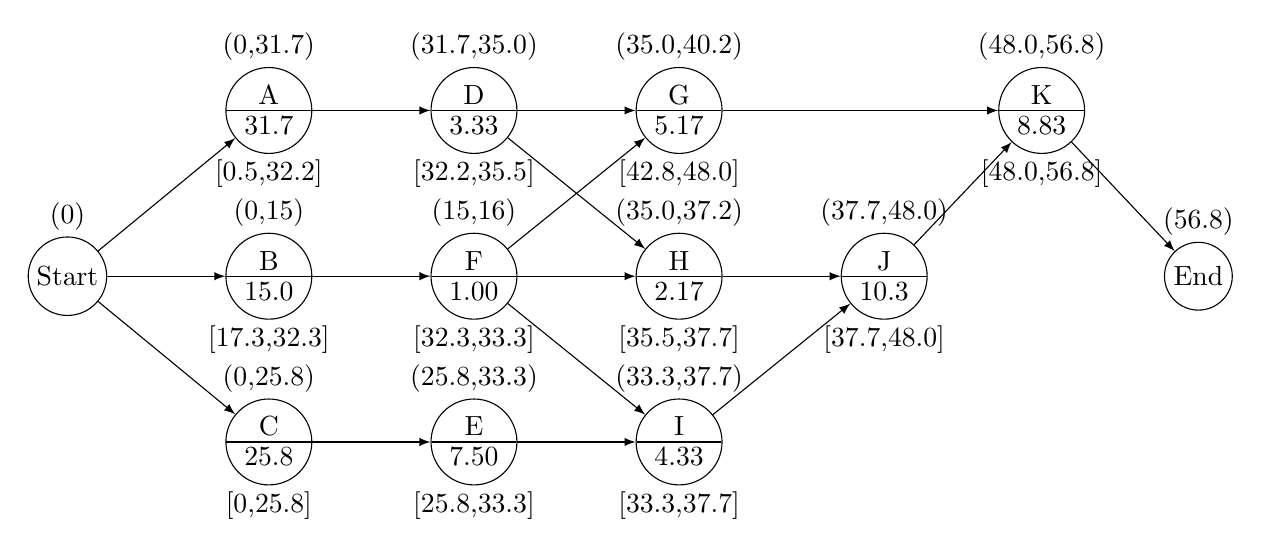
\begin{tikzpicture}[
  >=latex,
  every node/.style={draw,inner sep=2pt,minimum size=1pt},
  node distance=1.5cm,
  ]
  \node[circle, label=90:(0),] (S){Start};
  \node[circle split, right = of S, label=90:{(0,15)}, label=270:{[17.3,32.3]}] (B) {B \nodepart{lower} 15.0};
  \node[circle split, above = 1 of B, label=90:{(0,31.7)}, label=270:{[0.5,32.2]}] (A) {A \nodepart{lower} 31.7};
  \node[circle split, below = 1 of B, label=90:{(0,25.8)}, label=270:{[0,25.8]}] (C) {C \nodepart{lower} 25.8};
  \node[circle split, right = of A, label=90:{(31.7,35.0)}, label=270:{[32.2,35.5]}] (D) {D \nodepart{lower} 3.33};
  \node[circle split, right = of C, label=90:{(25.8,33.3)}, label=270:{[25.8,33.3]}] (E) {E \nodepart{lower} 7.50};
  \node[circle split, right = of B, label=90:{(15,16)}, label=270:{[32.3,33.3]}] (F) {F \nodepart{lower} 1.00};
  \node[circle split, right = of D, label=90:{(35.0,40.2)}, label=270:{[42.8,48.0]}] (G) {G \nodepart{lower} 5.17};
  \node[circle split, right = of F, label=90:{(35.0,37.2)}, label=270:{[35.5,37.7]}] (H) {H \nodepart{lower} 2.17};
  \node[circle split, right = of E, label=90:{(33.3,37.7)}, label=270:{[33.3,37.7]}] (I) {I \nodepart{lower} 4.33};
  \node[circle split, right = of H, label=90:{(37.7,48.0)}, label=270:{[37.7,48.0]}] (J) {J \nodepart{lower} 10.3};
  \node[circle split, right = 3.5cm of G, label=90:{(48.0,56.8)}, label=270:{[48.0,56.8]}] (K) {K \nodepart{lower} 8.83};
  \node[circle, right = 3cm of J, label=90:{(56.8)}] (End) {End};

  
  \draw [->] (S) -- (A);
  \draw [->] (S) -- (B);
  \draw [->] (S) -- (C);
  \draw [->] (A) -- (D);
  \draw [->] (B) -- (F);
  \draw [->] (C) -- (E);
  \draw [->] (D) -- (H);
  \draw [->] (D) -- (G);
  \draw [->] (F) -- (H);
  \draw [->] (F) -- (I);
  \draw [->] (F) -- (G);
  \draw [->] (E) -- (I);
  \draw [->] (H) -- (J);
  \draw [->] (I) -- (J);
  \draw [->] (J) -- (K);
  \draw [->] (G) -- (K);
  \draw [->] (K) -- (End);
  
\end{tikzpicture}

}
	\end{center}
	
	\pagebreak
	
	\subsection*{(b)}
	{\renewcommand{\arraystretch}{1.2} 
	\begin{table}[h!tbp]
  		\begin{center}
    		\caption{Slacks for Buying Tom Cruise a Boat}
    		\label{tab:table2}
			
    		\begin{tabular}{lcccccc}
				 & Total Slack Eq &  &  & Free Slack Eq & &\\
				Activity & LS - ES & = & Total Slack & Min\{ES$_{\text{Suc}}$\} - EF &= & Free Slack \\
				\hline
      			A  & 0.5-0  & = & 0.5  & 31.7-31.7 & = & 0 \\
      			B  & 17.3-0 & = & 17.3 & 15-15     & = & 0 \\
				C* &        &   & 0    &           &   & 0 \\
				D  & 32.2-31.7  & = & 0.5   & 35-35 & = & 0 \\
				E* &        &   & 0   &       &   & 0 \\
				F  & 32.3-15  & = & 17.3  & 33.3-16 & = & 17.3\\
				G  & 42.8-35  & = & 7.8   & 48-40.2 & = & 7.8 \\
				H  & 35.5-35  & = & 0.5   & 37.7-37.2 & = & 0.5 \\
				I* &        &   & 0   &       &   & 0 \\
				J* &        &   & 0   &       &   & 0 \\
				K* &        &   & 0   &       &   & 0 \\
				\hline
				\multicolumn{3}{c}{* = On the Critical Path}\\
    		\end{tabular}
  		\end{center}
	\end{table}
	}
	
	\noindent The slacks are slightly different, but the larger patterns still remain. Activities A,B, and D have some total slack, but none of it free. Activities F,G, and H have the same total slack and free slack, a pattern that continues from the previous estimate although the numbers have changed.
	
	\subsection*{(c)}
	\noindent Critical Path: C-E-I-J-K\\
	Mean Critical Path Time: 56.8 days\\
	Standard Deviation Critical Path: 3.31\\
	
	\noindent The critical path has not changed activities, but the mean time to complete has gone up.
	
	\subsection*{(d)}
	\subsubsection*{(1)}
	\begin{equation*}
		P\bigg(Z\le \frac{54-56.8}{3.31}\bigg) = 1 - P(Z \le 0.846) \cong 1 - 0.801 \approx 0.2
	\end{equation*}
	There is a 20\% chance that the project will be completed in 54 weeks or less.
	
	\subsubsection*{(2)}
	\begin{equation*}
		P\bigg(Z\le \frac{56.8-56.8}{3.31}\bigg) = P(Z \le 0) =  0.5
	\end{equation*}
	There is a 50\% chance that the project will be completed in the mean project time or less.
	
	\subsubsection*{(3)}
	\begin{equation*}
		P\bigg(Z\ge \frac{70-56.8}{3.31}\bigg) = 1 - P(Z \le 3.99) \cong 1 - 1 \approx 0
	\end{equation*}
	\begin{equation*}
		P\bigg(Z\ge \frac{64-56.8}{3.31}\bigg) = 1 - P(Z \le 2.18) \cong 1 - 0.985 \approx 0.015
	\end{equation*}
	There is a near 0\% chance that the project will take longer than 70 weeks to complete.\\
	There is a 1.5\% chance that the project will take 64 weeks or longer to complete.
	
\end{document}